% !BIB program = bibtex
% !TeX root = ../main.tex

\chapter{Problem Formulation}

In this chapter, we will introduce the scenario of the carpooling fairness problem. Then formulate the problem into a mathematical model with given parameters and decision variables.

\section{Problem Description}

The object of this research is to minimize the maximum percentage of cost saving when a passenger chooses to carpool, with consideration of the number of drivers, car capacity and routing limit constraints.

Take Figure 3-1 as an example scenario; Passenger 1 and Passenger 2 are requesting a trip. When Passenger 1 chooses to take a ride by himself/herself, called "exclusive" riding shown as Figure 3-2, it would cost \$5. We can describe the scenario as a shortest path problem from $S$ to $D_1$, and $P_1$ is a must-pass node. We use Steiner tree to solve this kind of shortest path problem with must-pass nodes. Passenger 2's "exclusive" riding would also cost \$5 in Figure 3-3. In this case, it would be a shortest path problem from $S$ to $D_2$ with $P_2$ as a must-pass node.

When the passengers choose to take a carpool, which is called "sharing" riding. We can describe the scenario as a shortest problem from $S$ to $D_1$ with $P_1$, $P_2$ and $D_2$ as must-pass nodes or $S$ to $D_2$ with $P_1$, $P_2$ and $D_1$ as must-pass nodes. In Figure 3-4 is one of the best case, which would cost \$8 for all the passengers, in Figure 3-5 would cost the same \$8 and both of the fares they could share are \$5 ( $\overline{P_2D_1}$ and $\overline{P_2D_2}$ respectively); however, in Figure 3-4 would cost $\overset{\overline{P_1P_2}}{1} + \frac{1}{2} \times \overset{\overline{P_2D_1}}{5} = \$3.5$ for Passenger 1 and $\frac{1}{2} \times \overset{\overline{P_2D_1}}{5} + \overset{\overline{D_1D_2}}{1} = \$3.5$ for Passenger 2, in Figure 3-5 would cost $\overset{\overline{P_1P_2}}{1} + \frac{1}{2} \times \overset{\overline{P_2D_2}}{5} + \overset{\overline{D_2D_1}}{1} = \$4.5$ for Passenger 1 and $\frac{1}{2} \times \overset{\overline{P_2D_2}}{5} = \$2.5$ for Passenger 2.

\begin{figure}[htp]
  \centering
  \captionsetup{justification=centering}
  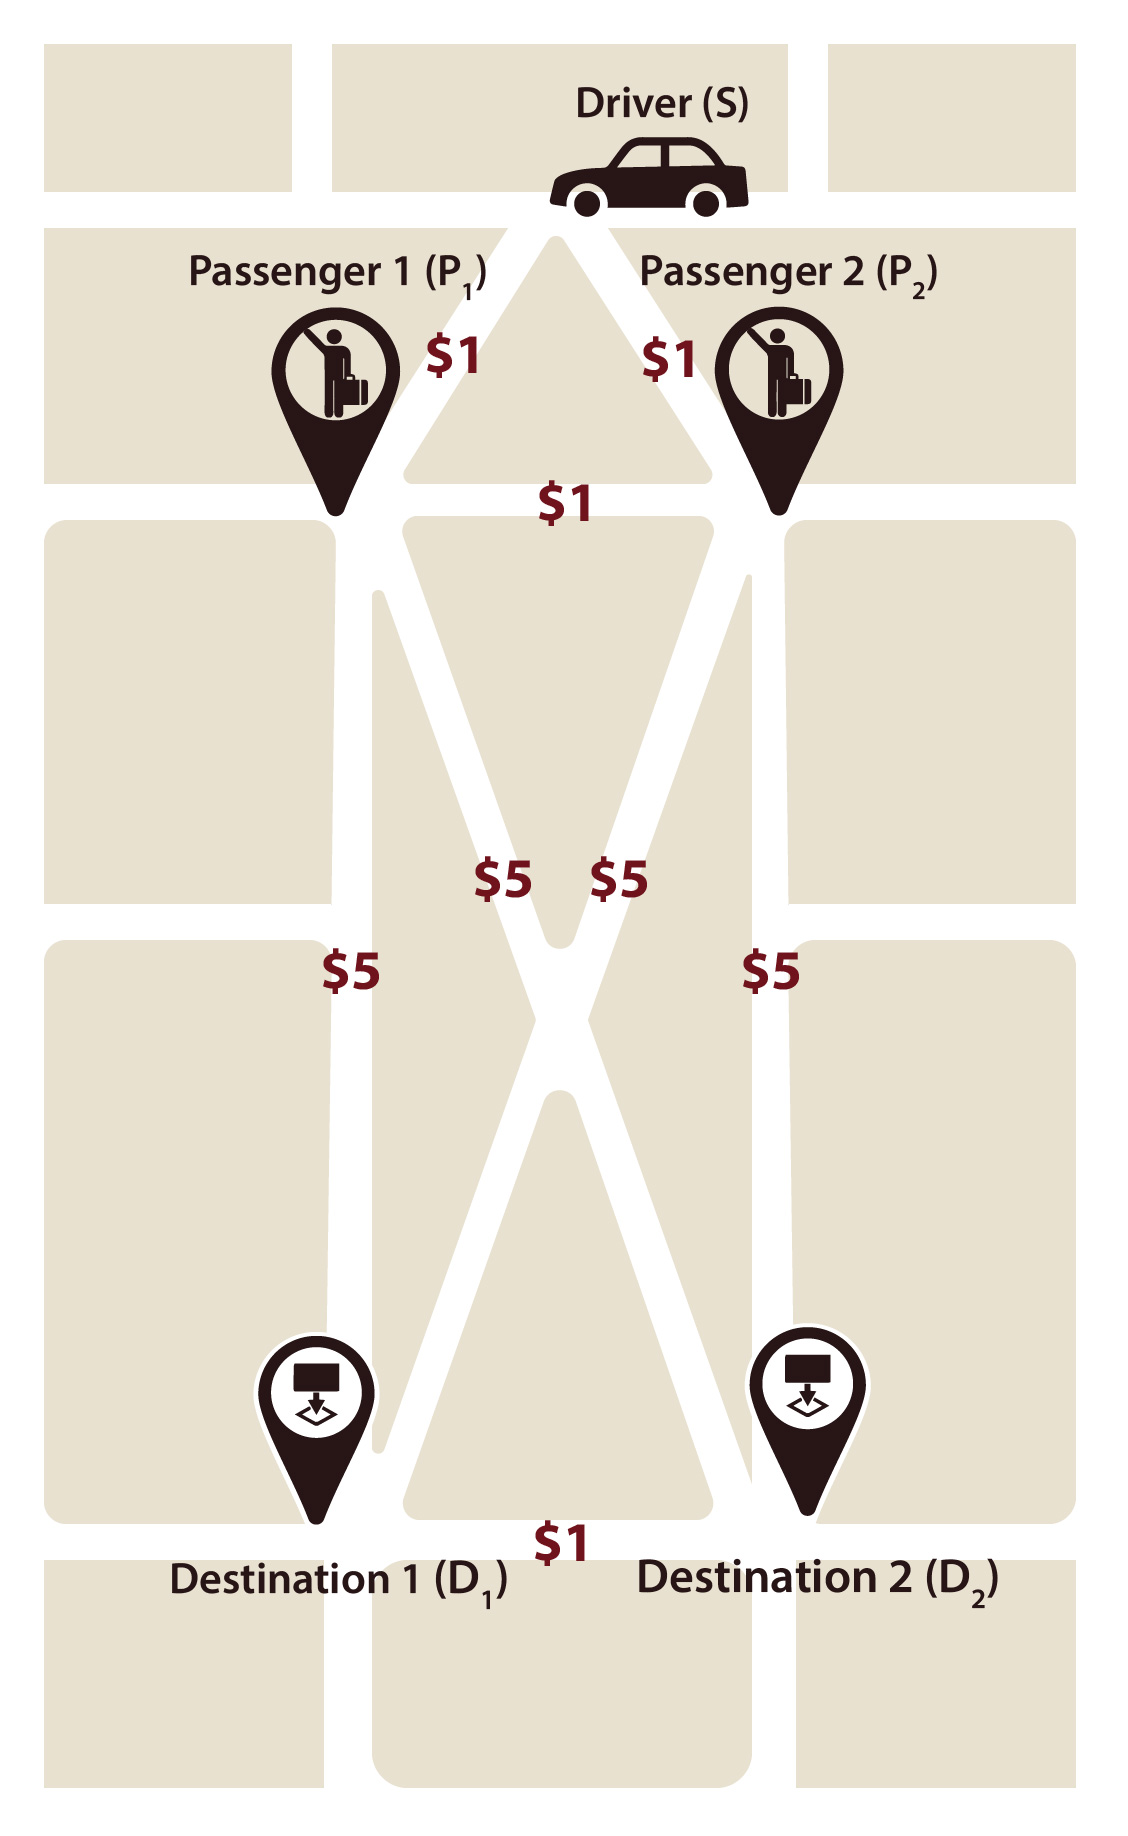
\includegraphics[width=6cm]{figures/mapV2.jpg}
  \caption{Example road network with driving fare and points of passengers and their destinations}
\end{figure}

\begin{figure}[htp]
  \centering
  \captionsetup{justification=centering}
  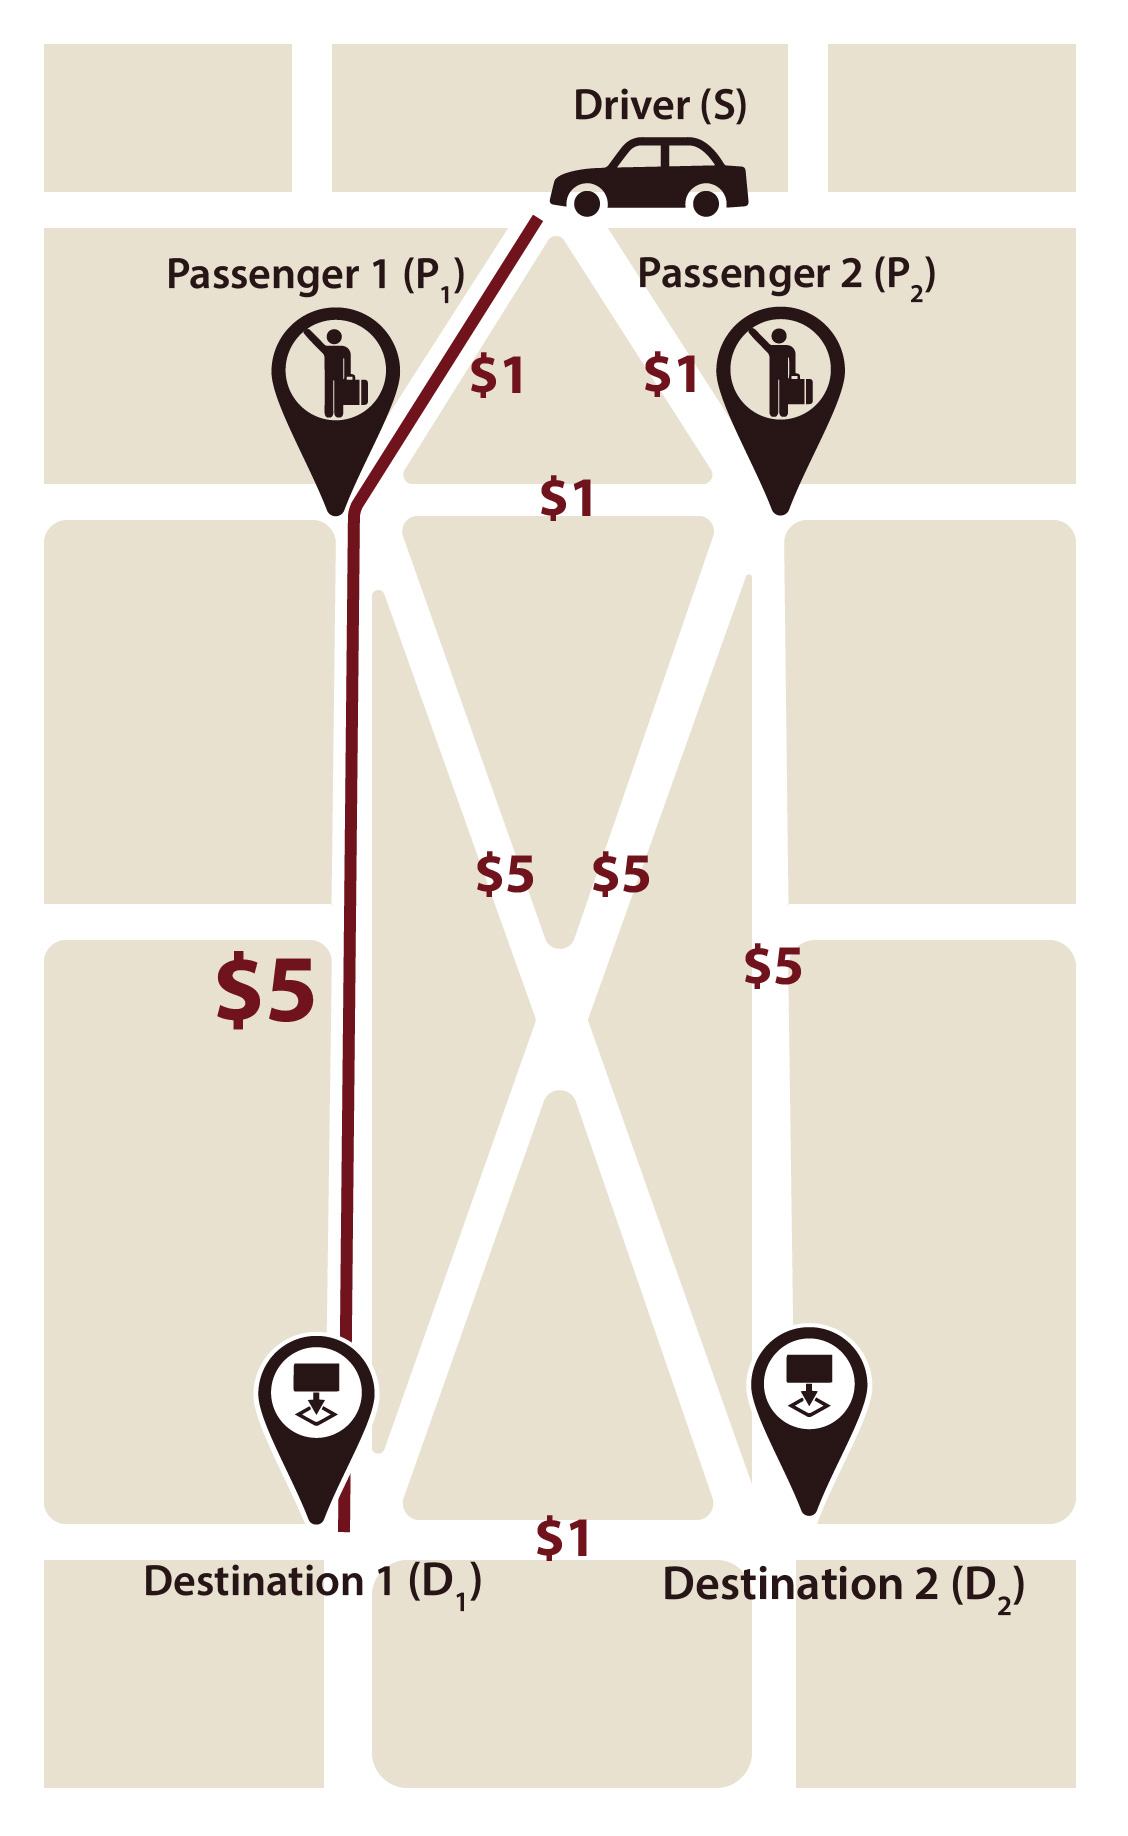
\includegraphics[width=6cm]{figures/mapV2_1.jpg}
  \caption{Best routing path when the driver only serving Passenger 1}
\end{figure}

\begin{figure}[htp]
  \centering
  \captionsetup{justification=centering}
  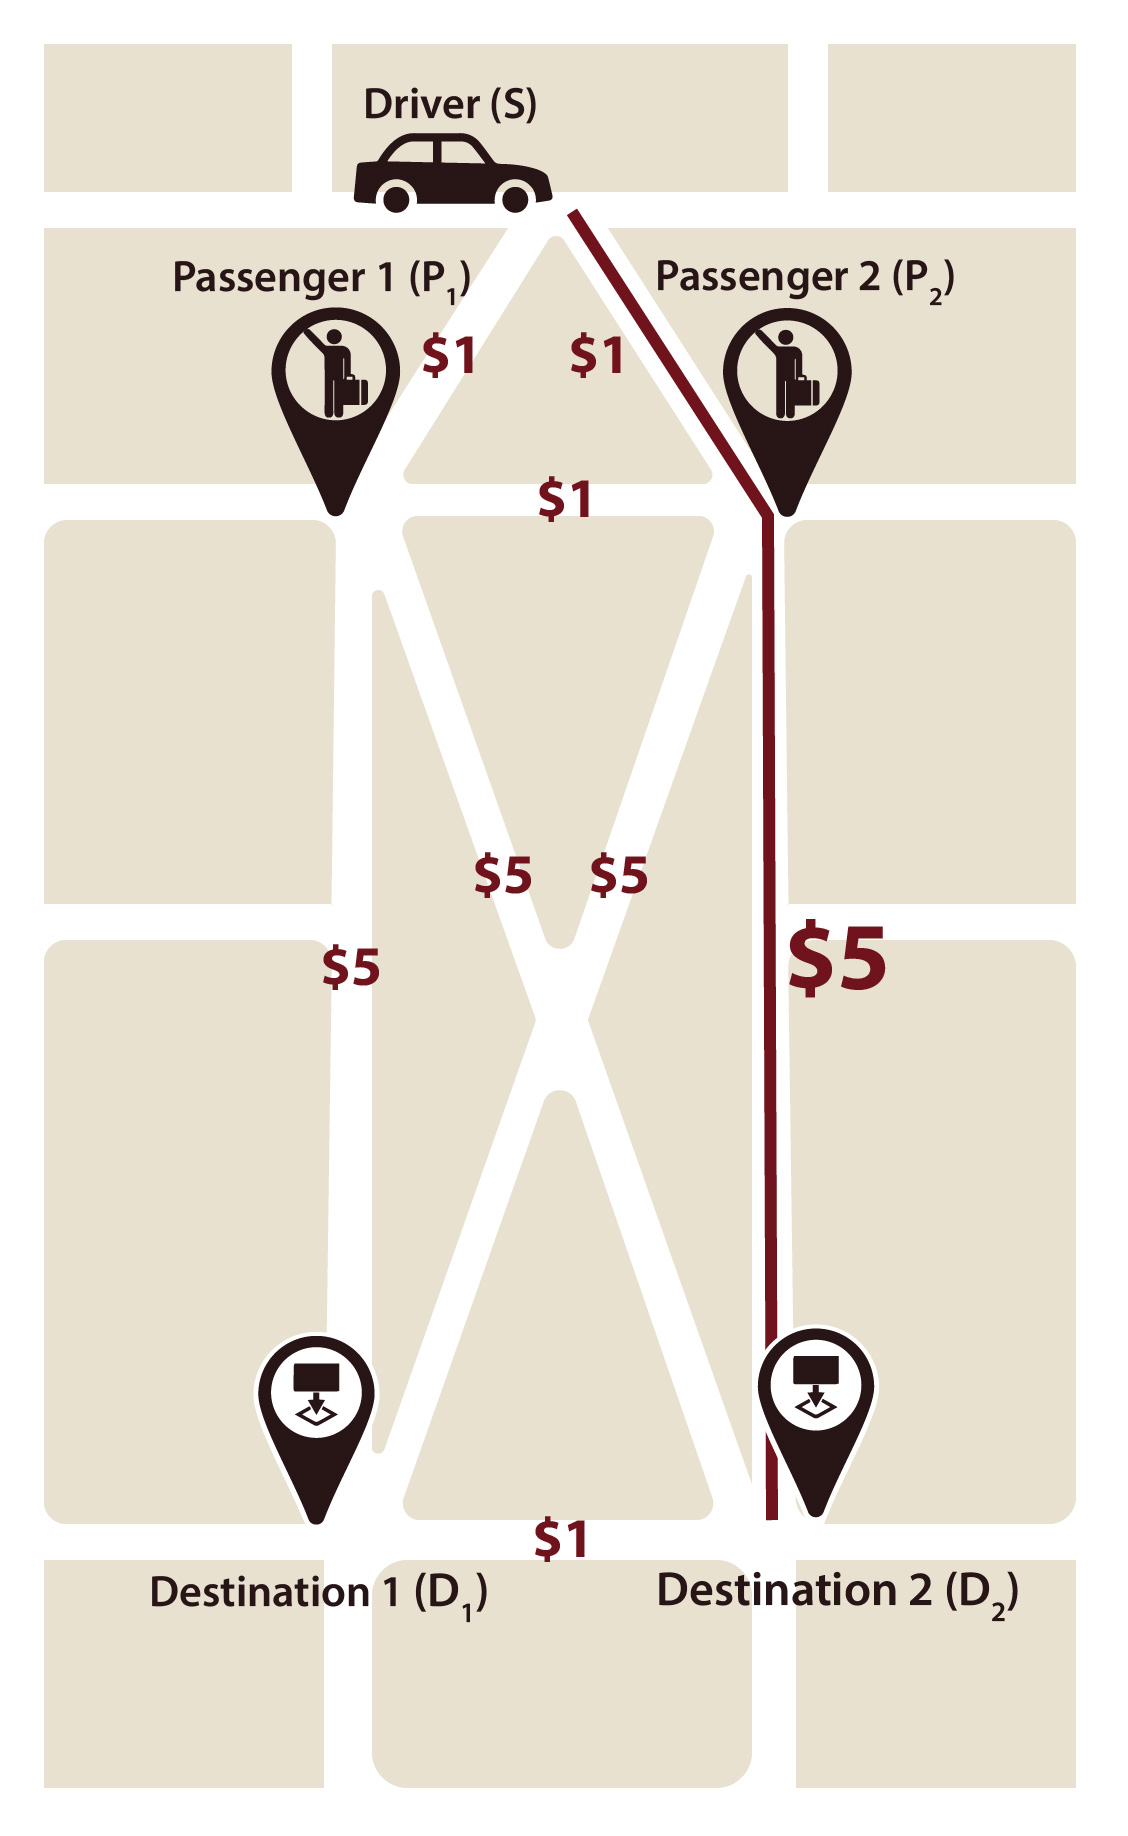
\includegraphics[width=6cm]{figures/mapV2_4.jpg}
  \caption{Best routing path when the driver only serving Passenger 2}
\end{figure}

\begin{figure}[htp]
  \centering
  \captionsetup{justification=centering}
  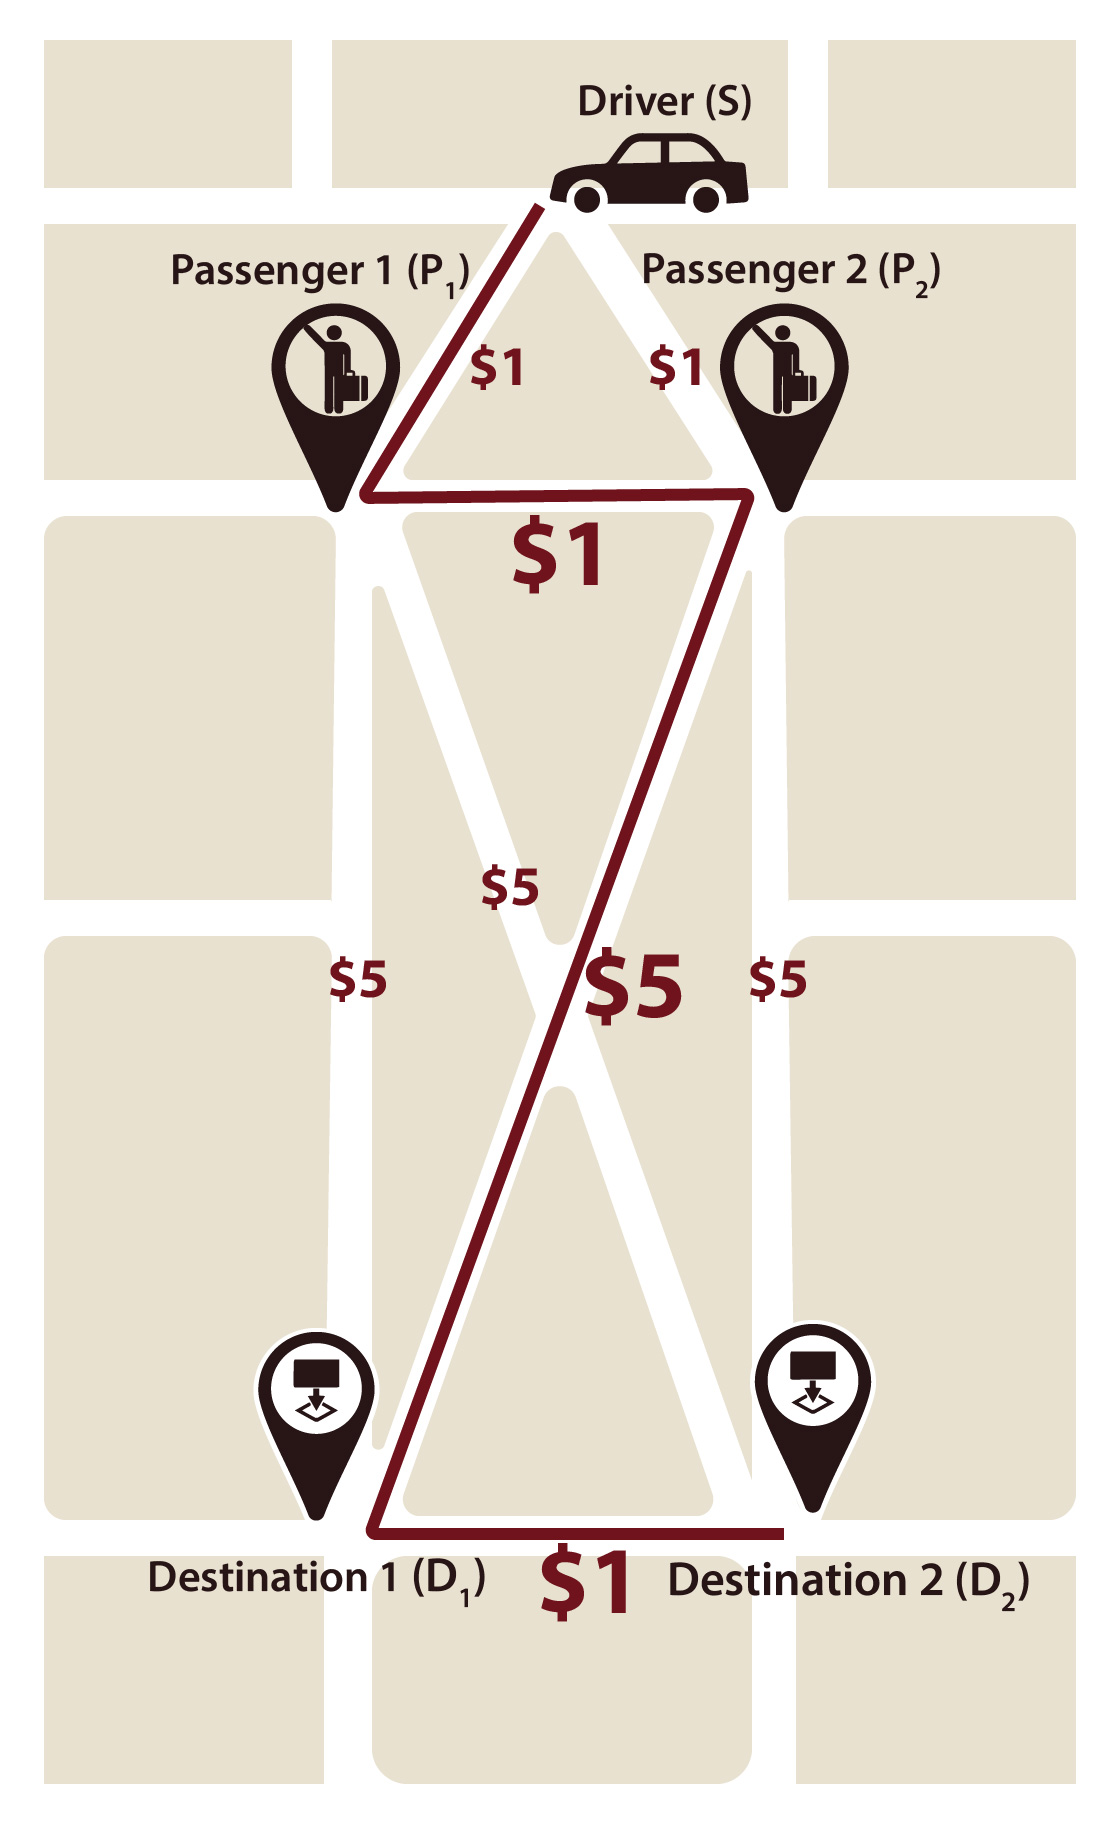
\includegraphics[width=6cm]{figures/mapV2_2.jpg}
  \caption{One of the best routing when both Passenger 1 and Passenger 2 carpool}
\end{figure}

\begin{figure}[htp]
  \centering
  \captionsetup{justification=centering}
  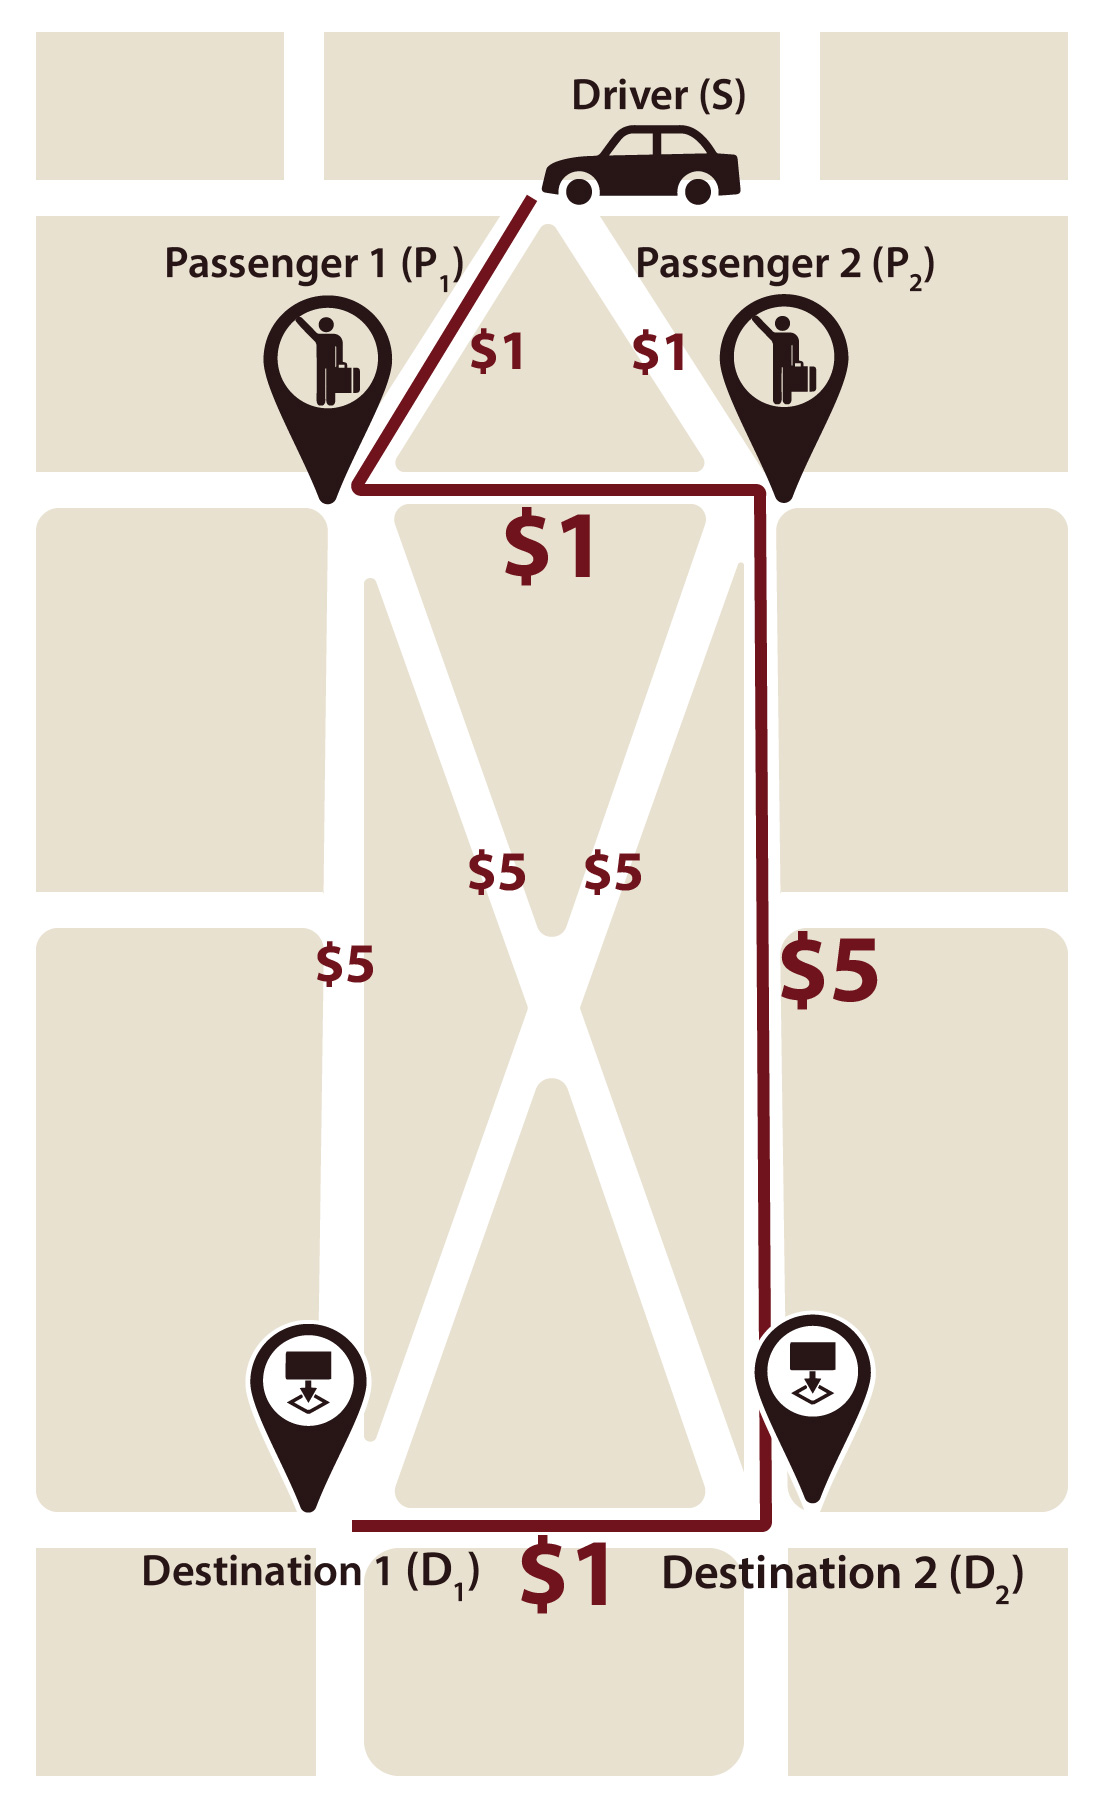
\includegraphics[width=6cm]{figures/mapV2_3.jpg}
  \caption{Another best routing when both Passenger 1 and Passenger 2 carpool}
\end{figure}
\newpage

\subsection{Assumptions}

There are three assumption in out system:

\begin{enumerate}
  \item System calculation time is not considered, that is, assume that drivers' location will still keep unchanged after the time of system calculation.
  \item The carpooling fare is shared equally by the time passengers in the vehicle. For a specific link in the route with $n$ passengers, the fare of the link for a passenger will be divided by $n$.
  \item All the passengers on the trip will accept the offer of carpooling.
  \item Total driving time is equal to sum of time spending of links that pass by.
 \end{enumerate}

\subsection{Fairness of Vehicle Dispatching}

In order to consider the fairness when dispatching driver, we introduce Jain's fairness index to avoid unfair situation:

$Firness\ Index = f_A(x) = \frac{\left(\sum\limits_{i=1}^{n} x_i\right)^2}{n \sum\limits_{i=1}^{n} x_i^2}$

We take accumulate driving requests that a driver has received as the metrics for fairness. That is, when a driver receives more driving requests in the past, he/she should give his/her chance of receiving a new driving request to the one who takes fewer driving requests.

As a new driving request comes, we need to ensure our system must get more or at least keep the same fairness. Hence, we form a constraint that the fairness index can not decrease compared to the previous fairness index.

However, when the driving resource changes, such as a new driver joins our system, it will violate our constraint for fairness. Because the newcomer has not taken any driving request before, the fairness will decrease. Even if a driver leaves our system, the fairness will increase or decrease due to the driver's situation. As a result, we need to reset the fairness index to the initial state and reset all the drivers' accumulated driving requests to 0. Nevertheless, it will make the fairness index's denominator to 0, which can not be divided. To avoid this situation, we assign a virtual driver with one accumulated driving request, which will make the fairness index to $\frac{1}{(n+1)}$, where $n$ is the number of drivers in our system. Moreover, for any situation that the fairness index will decrease when dispatching a new driving request, the fairness will reset.

\newpage

\section{Mathematical Model}

We will go through the detailed given parameters and decision variables in the mathematical model before describing our mathematical model.

The road network is represented as a weighted graph $G = (N, L)$, where $N$ is the nodes and $L$ is the links in the graph.

A riding request consists with following parameters: origin node, destination node, number of passengers, start time and deadline for driver to pick up.

\renewcommand\arraystretch{1.0}
\par
\begin{longtable}{cp{14cm}}
  \caption{Notations of given parameters}\\
  \toprule
  \multicolumn{1}{l}{Notation}&
  \multicolumn{1}{l}{Description}\\
  \midrule
  \endhead
    $C$ & Set of cab drivers in the system \\
    $R$ & Set of riding requests in the system (take $i$ as index) \\
    $R'$ & Set of riding requests which are not dispatched in current decision round, $R' \in R$ \\
    % $G_c$ & Set of riding requests that driver $c \in C$ has accepted but not arrived to the location of passengers in previous decision round. \\
    % $H_c$ & Set of riding requests that driver $c \in C$ has accepted and picked up in previous decision round. \\
    $O$ & Set of origin nodes of riding requests \\
    $D$ & Set of destination nodes of riding requests \\
    $N$ & Set of nodes on the road network, which include nodes of cab drivers, origin and destination nodes of riding requests, $N \in C \cup O \cup D$ \\
    $L$ & Set of links on the road network. A link can connect with any two nodes in the road network. \\
    $o_i$ & Origin node of riding request $i \in R$, $o_i \in O$ \\
    $d_i$ & Destination node of riding request $i \in R$, $d_i \in D$ \\
    $q_i$ & Number of passengers associates with riding request $i \in R$ \\
    $h_i$ & Maximum passengers limit of carpooling associates with riding request $i \in R$ \\
    $t_i$ & Remaining time to the start time of riding requesting $i \in R$ for driver to pick up in current decision round. \\
    $u_i$ & Remaining time to the deadline of riding requesting $i \in R$ for driver to pick up in current decision round. \\
    $T$ & Maximum additional buffer time to wait for pick up in the system. \\
    $Q_c$ & Maximum load capacity for driver, $c \in C$ \\
    $L_{O}$ & Set of artificial links of origin nodes \\
    $L_{D}$ & Set of artificial links of destination nodes \\
    $P_{co_i}$ & Set of paths from current location of driver $c \in C$ to origin node of riding request $i \in R$ \\
    $P_{cd_i}$ & Set of paths from current location of driver $c \in C$ to destination node of riding request $i \in R$ \\
    $P_c$ & Set of available paths from current location of driver $c \in C$ to a virtual node out of the road network. A virtual node is connected with all of nodes in the road network, with 0 weight links. \\
    $t_{cl}$ & The driving time for driver $c \in C$ on the link $l \in L$ \\
    $t_{ci}$ & The driving time of exclusive riding request $i \in R$ for driver $c \in C$ \\
    $f_{cl}$ & The fare rate for driver $c \in C$ on the link $l \in L$ \\
    $f_{ci}$ & The fare rate of exclusive riding request $i \in R$ for driver $c \in C$ \\
    $E$ & Maximum detour time ratio of hitchhiking for passengers in a riding trip. \\
    $\delta_{pl}$ & Indicator function which is 1 if link $l \in L$ on the route $p \in P_c \cup P_{co_i} \cup P_{cd_i}$ \\
    $a_c$ & Total fare that the driver $c \in C$ has earned before current decision round. \\
    $\alpha$ & The fairness index in the previous decision round. \\
  \bottomrule
\end{longtable}  
\par

\begin{longtable}{cp{14cm}}
  \caption{Notations of decision variables}\\
  \toprule
  \multicolumn{1}{l}{Notation}&
  \multicolumn{1}{l}{Description}\\
  \midrule
  \endhead
    $x_{p}$ & Binary variable, 1 if route $p \in P_{co_i}$ is chosen for driver $c \in C$; 0 otherwise. \\
    $y_{p}$ & Binary variable, 1 if route $p \in P_{cd_i}$ is chosen for driver $c \in C$; 0 otherwise. \\
    $z_{p}$ & Binary variable, 1 if route $p \in P_c$ is chosen for driver $c \in C$; 0 otherwise. \\
    $w_{ci}$ & Binary variable, 1 if riding request $i \in R$ is chosen for driver $c \in C$; 0 otherwise. \\
    $s_{cli}$ & Binary variable, 1 if link $l \in L \cup L_O \cup L_D, i \in R$ is passed by any driver $c \in C$ in carpooling; 0 otherwise. \\
  \bottomrule
\end{longtable}  
\newpage

\subsubsection*{Objective Function}

The objective function is to maximize the minimum discount percentage when applying carpooling among passengers in one trip.

\begin{align*}
  \max_{i \in R} \min_{c \in C} \frac{w_{ci} f_{ci} - carpool\ cost_c}{w_{ci} f_{ci}} \tag{IP1} \\
\end{align*}

\subsubsection*{Constraints}

\begin{align}
  \intertext{Constraint \eqref{waiting_time_start}, \eqref{waiting_time_end} ensures the pick up time is suit for the riding request.}
  & \sum\limits_{p \in P_{co_i}} \sum\limits_{l \in L} x_{p} \delta_{pl} t_{cl} \geq t_i - T && \forall c \in C, i \in R' \label{waiting_time_start} \\
  & \sum\limits_{p \in P_{co_i}} \sum\limits_{l \in L} x_{p} \delta_{pl} t_{cl} \leq u_i + T && \forall c \in C, i \in R' \label{waiting_time_end} \\
  \intertext{Constraints \eqref{path_limit_origin}, \eqref{path_limit_destination}, \eqref{path_limit} ensure there is only one path selected for a driver.}
  & \sum\limits_{p \in P_{co_i}} x_{p} \leq 1 && \forall c \in C, i \in R' \label{path_limit_origin} \\
  & \sum\limits_{p \in P_{cd_i}} y_{p} \leq 1 && \forall c \in C, i \in R' \label{path_limit_destination} \\
  & \sum\limits_{p \in P_{c}} z_{p} \leq 1 && \forall c \in C \label{path_limit} \\
  \intertext{Constraint \eqref{riding_request_limit} ensures a riding request only be assigned by at most one driver.}
  & \sum\limits_{c \in C} w_{ci} \leq 1 && \forall i \in R' \label{riding_request_limit}
  % \intertext{Constraint \eqref{previous_riding_request} ensures every riding requests a driver has picked up in previous round are assigned.}
  % & w_{ci} = 1 && \forall i \in G_c \cup H_c, c \in C \label{previous_riding_request}
  \intertext{Constraint \eqref{pick_up_drop_off_limit} ensures a riding request be picked up before dropping off.}
  & \sum\limits_{p \in P_{co_i}} \sum\limits_{l \in L} x_{p} \delta_{pl} t_{cl} \leq \sum\limits_{p \in P_{cd_i}} \sum\limits_{l \in L} y_{p} \delta_{pl} t_{cl} && \forall c \in C, i \in R' \label{pick_up_drop_off_limit} \\
  \intertext{Constraints \eqref{artificial_link_limit} ensure artificial links be passed by if the order associates with the link is assigned.}
  & s_{cli} = w_{ci} && \forall l \in L_O \cup L_D, i \in R', c \in C \label{artificial_link_limit} \\
  \intertext{Constraints \eqref{overlap_limit_route}, \eqref{overlap_limit_origin}, \eqref{overlap_limit_destination} ensure paths to origin or destination is overlapped with the carpooling path. }
  & \sum\limits_{p \in P_{c}} z_{p} \delta_{pl} w_{ci} = s_{cli} && \forall l \in L \cup L_O \cup L_D, i \in R', c \in C \label{overlap_limit_route} \\
  & \sum\limits_{p \in P_{co_i}} x_{p} \delta_{pl} \leq s_{cli} && \forall l \in L \cup L_O \cup L_D, i \in R', c \in C \label{overlap_limit_origin} \\
  & \sum\limits_{p \in P_{cd_i}} y_{p} \delta_{pl} \leq s_{cli} && \forall l \in L \cup L_O \cup L_D, i \in R', c \in C \label{overlap_limit_destination} \\
  \intertext{Constraint \eqref{capacity_limit} ensures that riding requests not exceed capacity of the cab}
  % & \sum\limits_{i \in R' \cup H_c} \sum\limits_{p \in P_{cd_i}} y_{p} \delta_{pl} w_{ci} q_i - \sum\limits_{i \in R' \cup H_c} \sum\limits_{p \in P_{co_i}} x_{p} \delta_{pl} w_{ci} q_i \leq Q_c && \forall l \in L, c \in C \label{capacity_limit} \\
  & \sum\limits_{i \in R'} \sum\limits_{p \in P_{cd_i}} y_{p} \delta_{pl} w_{ci} q_i - \sum\limits_{i \in R'} \sum\limits_{p \in P_{co_i}} x_{p} \delta_{pl} w_{ci} q_i \leq Q_c && \forall l \in L, c \in C \label{capacity_limit} \\
  \intertext{Constraint \eqref{detour_ratio_limit} ensures detour time ratio of carpooling to exclusive riding for every riding requests not be larger than limit of the system.}
  & \frac{\sum\limits_{p \in P_{cd_i}} \sum\limits_{l \in L} y_{p} \delta_{pl} w_{ci} t_{cl} - \sum\limits_{p \in P_{co_i}} \sum\limits_{l \in L} x_{p} \delta_{pl} w_{ci} t_{cl}}{w_{ci} t_{ci}} \leq E && \forall c \in C, i \in R' \label{detour_ratio_limit} \\
  \intertext{Constraint \eqref{custom_capacity_limit} ensures that riding requests not exceed capacity limit of the riding request}
  % & \sum\limits_{i \in R' \cup H_c} \sum\limits_{p \in P_{cd_i}} y_{p} \delta_{pl} w_{ci} q_i - \sum\limits_{i \in R' \cup H_c} \sum\limits_{p \in P_{co_i}} x_{p} \delta_{pl} w_{ci} q_i \leq h_i && \forall l \in L, c \in C \label{custom_capacity_limit}
  & \sum\limits_{i \in R'} \sum\limits_{p \in P_{cd_i}} y_{p} \delta_{pl} w_{ci} q_i - \sum\limits_{i \in R'} \sum\limits_{p \in P_{co_i}} x_{p} \delta_{pl} w_{ci} q_i \leq h_i && \forall l \in L, c \in C \label{custom_capacity_limit}
  % \intertext{Constraint 3.7 ensures the fairness index after current decision round will not less than the previous decision round.}
  % & \frac{\left(\sum\limits_{r \in R} b_r\right)^2}{\sum\limits_{r \in R} 1 \sum\limits_{r \in R} b_r^2} \geq \alpha \\
  % \intertext{Constraint 3.8 is the fairness index in the previous decision round.}
  % & \frac{\left(\sum\limits_{r \in R} a_r\right)^2}{\sum\limits_{r \in R} 1 \sum\limits_{r \in R} a_r^2} \leq \alpha \\
\end{align}
